\documentclass{article}
\usepackage[utf8]{inputenc}
\usepackage[a4paper, left=20mm, top=15mm, right=20mm, bottom=15mm]{geometry}
\usepackage{graphicx}
\usepackage{enumitem}
\usepackage{amsmath} 
\usepackage{amssymb}
\usepackage{tikz}
\usepackage{pgfplots}

\newcommand{\resposta}{\hfill\makebox[0pt][r]{\scriptsize\textit{Resposta:\rule{5cm}{.1pt}}}\\ \vspace{.1cm}}
\newcommand{\um}{(1,0 ponto) }
\newcommand{\dois}{(2,0 pontos) }
\newcommand{\tres}{(3,0 pontos) }
\newcommand{\cinco}{(5,0 pontos) }
\begin{document}
\pagestyle{empty}

%\begin{figure}[!h]
%	\centering
%	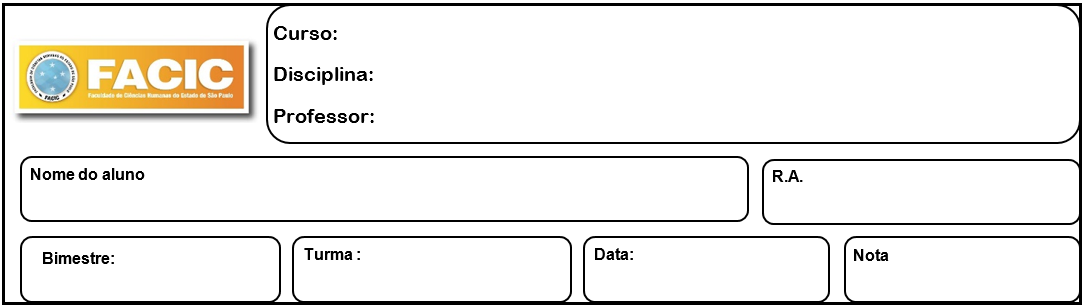
\includegraphics[width=1\linewidth]{cabecalho_FACIC}
%\end{figure}

%\vspace{-5.25cm}\hspace{5.5cm}{\textbf{ADMINISTRAÇÃO e CIÊNCIAS CONTÁBEIS}}

%\vspace{.21cm}\hspace{6.1cm}{\textbf{ÁLGEBRA LINEAR}}

%\vspace{.25cm}\hspace{6.1cm}{\textbf{FUMACHI}}

%\vspace{2.1cm}\hspace{1.1cm}{\textbf{2º Bimestre}}
%\hspace{6.3cm}{\textbf{}}

%\vspace{0.4cm}
\begin{center}\textbf{\Large{Disciplina de Matemática - 1 Adm e 1 CC \\ Prof. Fumachi \\ \vspace{0.5cm} Atividade 02}}\end{center}
\begin{center}\large{Data limite de entrega: 04/04/2020}\end{center}
%\textbf{Orientações:}
%\begin{enumerate}[label=\alph*,nosep]
%	\item[a)]{A avaliação é INDIVIDUAL;}
%	\item[b)]{NÃO é permitido a comunicação com outros colegas/amigos durante a avaliação;}
%	\item[c)]{NÃO é permitido durante a avalição utilizar qualquer equipamento elétrico, eletrônico, EXCETO calculadora PRÓPRIA;}
%	\item[d)]{NÃO é permitido emprestar materiais dos e/ou para os colegas, mesmo que tenha terminado a avaliação;}
%	\item[e)]{O não cumprimento de um, ou mais, dos itens (a-d), acarretará na anulação da avaliação e será atribuída a nota 0 (zero);}
%	\item[f)]{O entendimento da questão/enunciado faz parte da avaliação, ou seja, não haverá explicações do professor;}
%	\item[g)]{As respostas das questões devem ser feitas apenas no espaço destinado a mesma e devem ser feitas a tinta (preta ou azul). Respostas com rasuras, não legíveis ou feitas a grafite serão anuladas.}
%\end{enumerate}
	
\par\noindent\rule{\textwidth}{1pt}
%\textbf{{Questões}}

\vspace{0.25 cm}

\noindent 1. Calcule as raízes das funções abaixo:
\begin{itemize}
	\item[a.]{$f(x)=x^2-5x+6$}
	\item[b.]{$f(x)=-3x^2+15x+18$}
	\item[c.]{$f(x)=x^2-4x+4$}
	\item[d.]{$f(x)=-2x^2+8x-8$}
	\item[e.]{$f(x)=2x^2-12x+26$}
	\item[f.]{$f(x)=-4x^2+24x-52$}
\end{itemize}

\noindent 2. Calcule o vértice das funções do exercício 1.

\noindent 3. Faça o gráfico das funções do exercício 1.

\noindent 4. Com a propagação do SARS-CoV-2 e suas infecções causadas, é importante tomar cuidado e se prevenir! Vamos supor que um indivíduo infectado transmita o vírus para outras três pessoas em um dia. Suponha que cada pessoa infectada pelo primeiro indivíduo infecte, também, outras três pessoas por dia. Isso se repete sempre para cada indivíduo. Sabendo desse processo, determine:
\begin{itemize}
	\item[a.]{A função que descreve o número de indivíduos infectados em função do tempo;}
	\item[b.]{Quantos indivíduos estarão infectados após 10 dias?}
	\item[c.]{Supondo uma população de 220 milhões de pessoas, em quanto tempo todos estarão infectados?}
\end{itemize}
%\vspace{12.5cm}
%\resposta
%--------------------------------------

%\noindent 2. Classifique as sentenças abaixo em Verdadeiro (V) ou Falso (F):
%\vspace{.3cm}
%\begin{enumerate}[label=\alph*,nosep]
%	\item[2.1.]{(\qquad) O elemento neutro da soma de matrizes é a matriz nula.}
%	\item[2.2.]{(\qquad) O elemento neutro da multiplicação de matrizes é a matriz identidade.}
%	\item[2.3.]{(\qquad) A matriz identidade é uma matriz quadrada onde os elementos da diagonal principal são iguais a 1 e o restante iguais a 0.}
%	\item[2.4.]{(\qquad) Um sistema linear quando possui solução única ele é chamado de Sistema Possível e Determinado.}
%	\item[2.5.]{(\qquad) Um sistema linear pode ser classificado como SPI, SPD e SI.}
%	\item[2.6.]{(\qquad) O método de Cramer para resolver sistemas lineares possui falhas.}
%	\item[2.7.]{(\qquad) O método de Gauss para resolver sistemas lineares é conhecido, também, como método do escalonamento.}
%	\item[2.8.]{(\qquad) A matriz ampliada é usada no método de Gauss.}
%	\item[2.9.]{(\qquad) Na regra de Cramer, a matriz principal é uma matriz composta pelos coeficientes de um sistema linear.}
%	\item[2.10.]{(\qquad) O objetivo do método de Gauss para resolver sistemas lineares é obter uma matriz triangular inferior.}
%\end{enumerate}
%--------------------------------------

%\vspace{1cm}
\par\noindent\rule{\textwidth}{1pt}
Fim da Atividade 02.


\end{document}